\documentclass[12pt,letterpaper]{article}


\newcommand{\doctitle}{Scientific Computing Homework 3}
\newcommand{\docauthor}{Matthew Duschenes}
\newcommand{\docaffil}{Department of Applied Physics, University of Michigan}
\newcommand{\docheader}{NERS 570 \ - Homework 3 - \docauthor}
\newcommand{\docfooter}{\docaffil}


% Margins
\usepackage[margin=0.75in,marginparsep=0pt,paperwidth=216mm,paperheight=279mm]{geometry}

% Headers
\usepackage{fancyhdr}
\geometry{headheight=15pt}
\renewcommand{\headrulewidth}{0.4pt}% default is 0.4pt
\renewcommand{\footrulewidth}{0.4pt}% default is 0pt
\geometry{headheight=15pt}
\geometry{headsep=10pt}
\setlength{\skip\footins}{10pt} % gap between text and footer
\fancyhf{}
\fancyhead[R]{\docheader}
\fancyfoot[LE,RO]{\thepage}
\fancyfoot[LO,RE]{\docfooter}

% \makeatletter
% \if@twoside
% \fancyfoot[LE,RO]{\thepage}
% \fancyfoot[LO,RE]{\docfooter}
% \else
% \fancyfoot[R]{\thepage}
% \fancyfoot[L]{\docfooter}
% \fi
% \makeatother
% \fancyhead[R]{\docheader}


% Title
\usepackage{titling}
% \usepackage[affil-it]{authblk}
\usepackage[nodayofweek]{datetime}
\usepackage[super]{nth}

% \newdateformat{monthdayyear}{%
%   \monthname[\THEMONTH]~\THEDAY,~ \THEYEAR}
% \newdateformat{mydate}{\monthname[\THEMONTH] \nth[\THEDAY], \THEYEAR}


% Make Title
\pagestyle{fancy}
% \renewcommand*{\Authfont}{\bfseries}
% \renewcommand*{\Affilfont}{\normalfont\itshape}
\pretitle{\begin{center}\vskip -50pt}%
\title{\large \doctitle}
\posttitle{\end{center}}
\preauthor{\begin{center} \vskip -20pt}
\author{}
\postauthor{\end{center} \vskip -20pt}
\predate{\begin{center} \vskip -20pt}
\date{}%\small{\today}}
\postdate{\end{center} \vskip -20pt}% -42.5pt


% Fonts
\usepackage[singlespacing]{setspace}

 
% Math
\usepackage{amsmath}
\usepackage{amssymb}
\usepackage{physics}


% Figures
\usepackage{floatrow}
\usepackage{multicol}
\usepackage{grffile}
\usepackage{caption}
\usepackage{subcaption}
\usepackage{graphicx,xcolor}
\PassOptionsToPackage{export}{adjustbox}

% HypperReferences
\usepackage[pdftex,draft=false]{hyperref}
\hypersetup{
    colorlinks=true,
    linkcolor=black,
    citecolor=black,
    urlcolor=black}
\usepackage{url}

% References
\usepackage[capitalize]{cleveref}


% Code
\usepackage{minted}
\renewcommand\listingscaption{Code}
\floatsetup[listing]{style=Plaintop}    

\crefname{listing}{Code.}{Code}
\newminted{python}{frame=lines,framerule=2pt,float=ht}
\setminted{breaklines,frame=single,framesep=2pt,breakindent=10pt,breakafter={,},breaksymbolleft=}

\newenvironment{longlisting}{\captionsetup{type=listing}}{}
\newcommand{\code}[4]{
% \begin{listing}[ht]
\begin{longlisting}
    \caption{#3}
    \inputminted{#1}{#2}
    \label{code:#4}
\end{longlisting}
% \end{listing}
}


 % Commands
\newcommand{\reals}{\mathbb{R}}
\DeclareMathOperator*{\argmax}{arg\,max}
\DeclareMathOperator*{\argmin}{arg\,min}

\newcommand{\eqtxt}[1]{\overset{#1}=}
\newcommand{\repo}[2]{\href{https://github.com/bkochuna/ners570f20-Lab06/#1/#2}{\##2}}


%%%%%%%%%%%%%%%%%%%%%%%%%%%%%%%%%%%%%%%%%%%%%%%%%%%
\begin{document}
\maketitle
\thispagestyle{fancy}
\singlespacing
%%%%%%%%%%%%%%%%%%%%%%%%%%%%%%%%%%%%%%%%%%%%%%%%

\section{Ex4 - Monte Carlo Simulations}

\subsection{Code Description}
A \textit{Spin} class is created in C++ to simulate spin systems on a lattice using Markov-Chain Monte Carlo (MCMC) in $d$ dimensions, and with spin systems that can be in $q$-fold states. This class contains functions to setup the lattice, setup the physical system (at system size $n$, temperature $T$, number of spin states $q$, and coupling fields $J$), and set settings for the MCMC simulations. All classes are templated by datatype, allowing for integer/nnon-integer spin values, and float/double precision observables. All code can be found in the appendix.

The MCMC simulation settings, contained in a C++ structure, include the maximum number of iterations, the seed for the random number generator, the burnin time of MCMC iterations before statistics are collected, and the settings whether to be verbose, or to save and write statistics to file. The class then contains a \textit{montecarlo} function that performs MCMC iterations by choosing random spins to flip to different spin values, and calculates the difference in energy of the states, which is strictly a local energy calculation at that chosen spin site. The acceptance probability is then used to determine whether to accept or reject this updated state, and then proceed to the next MCMC iteration. 

Please note, the transition probability is believed to be incorrect in the assignment, it should be the Boltzmann distribution $\sim e^{-\Delta E/T}$, not the Planck distribution $\sim \frac{1}{1+e^{-\Delta E/T}}$, however perhaps it was intended that there are slightly different conditions for this probability value.

The class contains functions to update the state of the system, contained in a C++ structure, which is a one dimensional array \textit{state} of spins of length $N = n^d$, which can be accessed by a linear index. The nearest neighbours to each index are contained in a pre-allocated two dimensional array of neighbours, of length $N \times z$, where $z = 2d$ is the coordination number for a square lattice in $d$ dimensions. 

The class also contains functions to update the observables for a given spin state of the system, including the energy $E$ and order $S$, as well as keeps a running average $\mu$ and (unbiased) variance $\sigma^2$ in the mean of each observable over the $M$ MCMC updates to the system. These are also included in a C++ structure, and have associated functions to calculate the observables locally at each spin, and globally across the lattice. Observables are defined as being normalized to be the quantities per spin. Here, slight variations of the variances are calculated, normalized by power of temperature, to give the specific heat, and the susceptibility for the energy and order respectively.

After $M$ MCMC iterations, for observables $\Omega$:
\begin{align}
  \mu_{\Omega}^{(M)} &\equiv \frac{1}{M} \sum_m \Omega^{(m)} \\
  \sigma_{\Omega}^2 &\equiv \frac{1}{M-1} \sum_m \left[ {\mu_{\mu_{\Omega}}^{(m)}}^2 - {\mu_{\mu_{\Omega}}^{(M)}}^2 \right]
\end{align}

A separate I/O class is also created in C++, to write out and read in data with headers to \textit{csv} files, and is templated to read and write in different data types.

A separate plotting class is also created in python, to visualize the statistics over the MCMC iterations.

\subsection{OpenMP Parallelization}
For parallelization of the MCMC with shared memory openMP, it is not embarrassingly parallel because the MCMC states are directly dependent on the previous states, and so each iteration cannot be run in parallel. Instead, the MCMC is stated to be parallel (\#pragma omp parallel for default(shared) private(i) shared(state,observables,settings)), however with shared \textit{state}, and \textit{observable} variables, and importantly \textit{critical} (\#pragma omp critical) clause is used  for most of the scope of the iteration, due to the state not being able to be updated in parallel, however some of the iteration can be parallelized, like calculating the transition probability.

To aid in speedup, the loops to calculate the observables across all spins are parallelized with (\#pragma omp for), with the \textit{state}, and \textit{observable} variables being shared again to hopefully avoid race conditions. The nearest neighbours array is also parallelized when it is initially defined in the class initialization.

These parallelizations, particularly because of the use of \textit{critical} do not appear to speed up the MCMC greatly, even for system sizes up to $n=100$ and $q=5$ and maximum iterations of $10^6$. However, the implementation already appears to be quite fast, and the resulting plots appear to show the correct physical behaviour at temperatures above and below the transition temperature $T_c$. In $d=2$, 

\begin{align}
  T_c = \frac{1}{\log{1+\sqrt{q}}}
\end{align}


A Makefile is used, to compile the C++ code, where the \textit{main.cpp} executable is dependent on the \textit{physics.cpp} and \textit{io.cpp} files. The GNU g++ compiler is used, with the the \textit{-fopenpm}, and each source file is compiled separately as object files, before being linked together. The Makefile also contains targets to run and plot the MCMC results, with input arguments of $n$, $q$, $T$, $J$. 

\subsection{MCMC Stopping Conditions}
For the MCMC stopping conditions, there are various methods of determining when the system has equilibrated at its given temperature. A simple approach is from determining the correlations between states after many MCMC iterations, and seeing at which point, the states are uncorrelated, and have reached an equilibria for its total energy per spin. The spin correlations can be found by taking the variance of the order parameter (average magnetization per spin), and the energy equilibration can be found by the taking the variance of the average energy of the system. These can be computed from the most recent $m$ MCMC iterations, and computed after the initial burnin iterations, to get an estimate for these quantities at the current iteration. Tolerances are placed on these variances, and if the calculated average variances over the previous $m$ MCMC iterations, then the equilibration has been said to have been reached and the MCMC can stop.


\subsection{Results}
Here are the following results for MCMC for $n=10$, $q=2$ (Ising Model), $T=\{0.5,T_c=1.31459,5\}$, for $J = 1$.


\begin{figure}[ht]
  \centering
    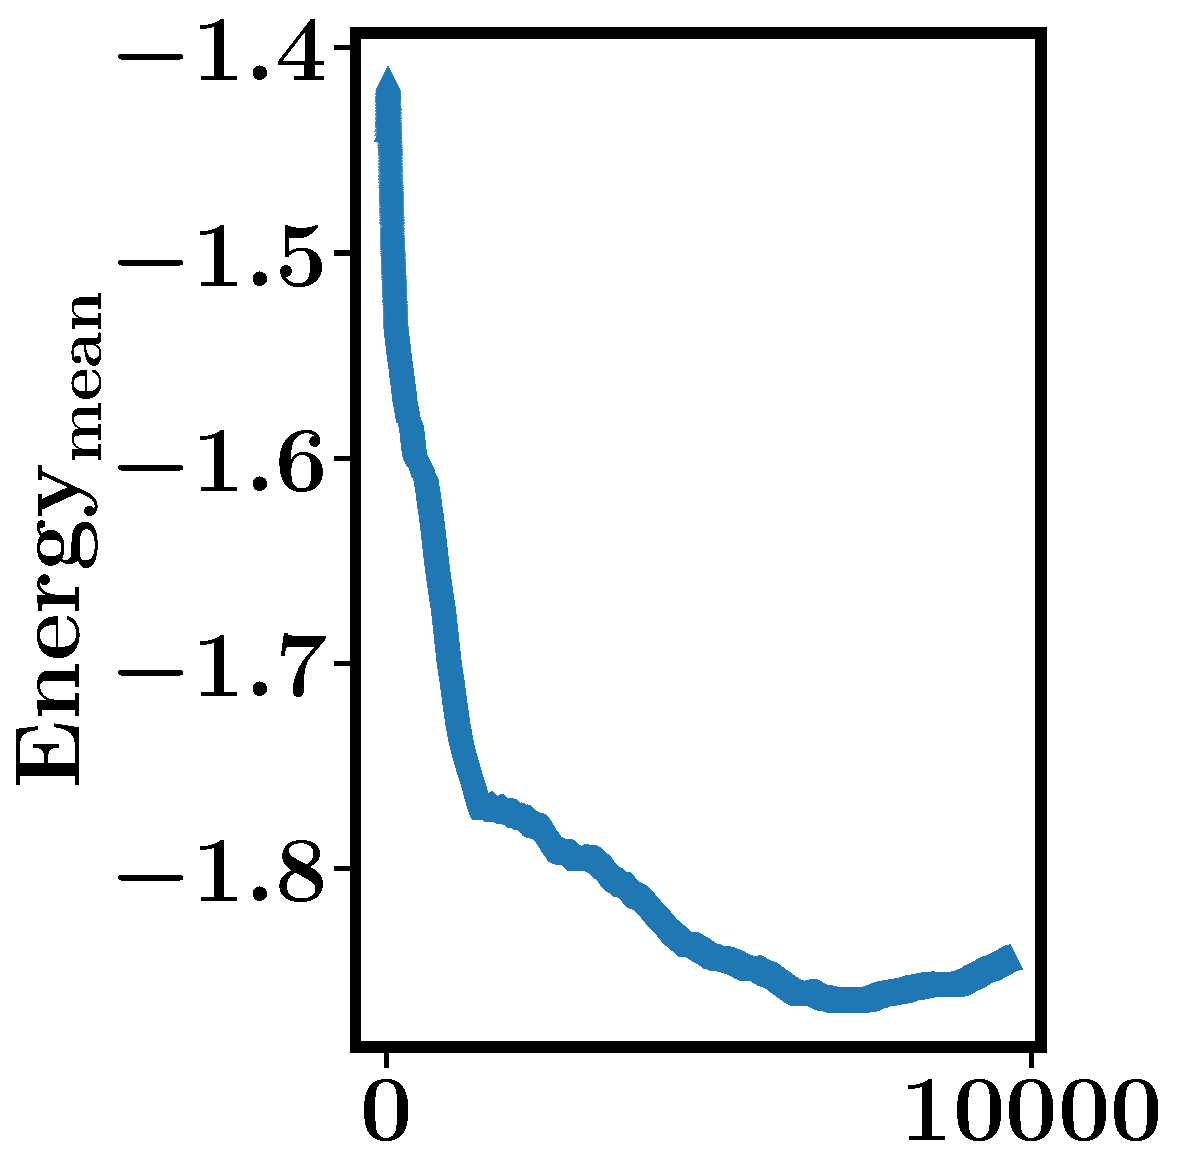
\includegraphics[width=\textwidth]{figures/plot_energy_T0-5.pdf}
    \caption{Average energy for $T = 0.5 < T_c$.}
     \label{fig:E0.5}
\end{figure}


\begin{figure}[ht]
  \centering
    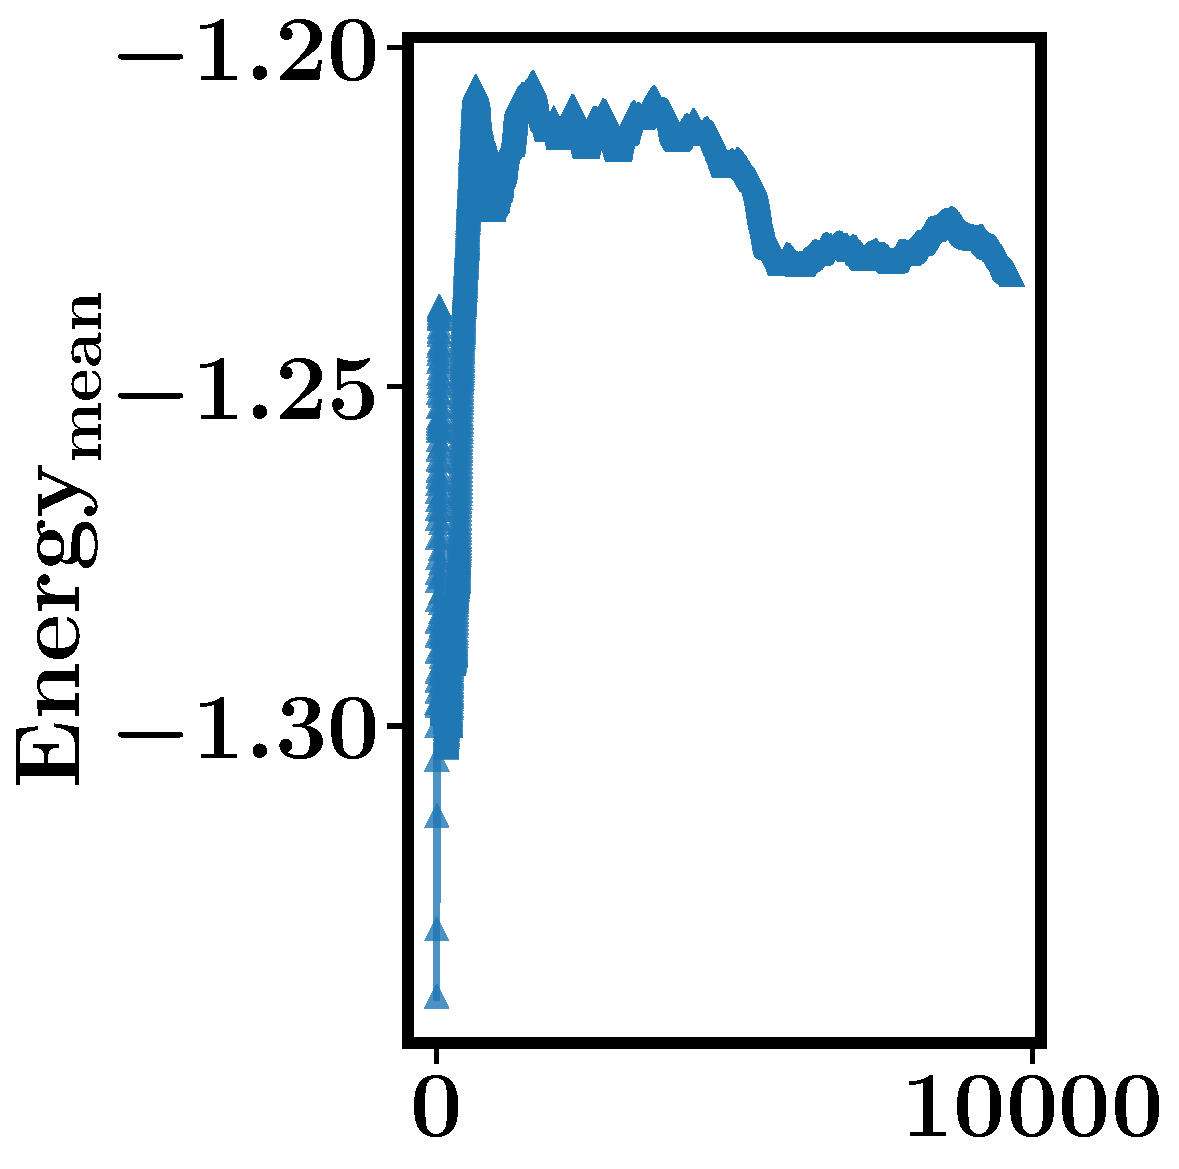
\includegraphics[width=\textwidth]{figures/plot_energy_T1-134593.pdf}
    \caption{Average energy for $T = 1.134593 = T_c$.}
     \label{fig:E0.5}
\end{figure}


\begin{figure}[ht]
  \centering
    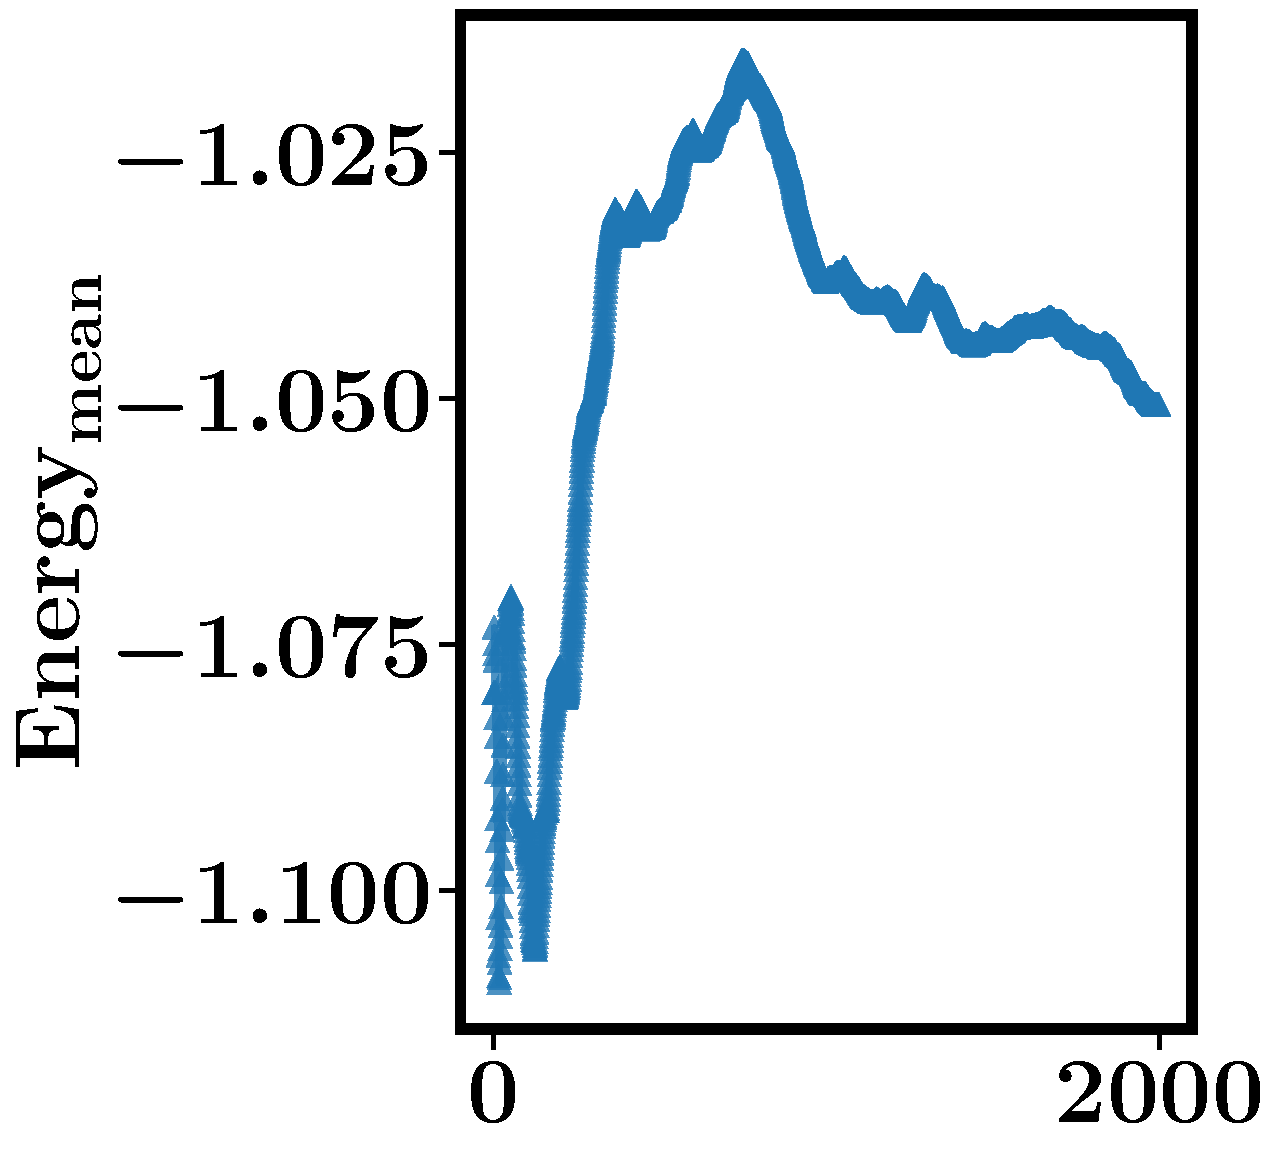
\includegraphics[width=\textwidth]{figures/plot_energy_T5.pdf}
    \caption{Average energy for $T = 5 > T_c$.}
     \label{fig:E0.5}
\end{figure}



\begin{figure}[ht]
  \centering
    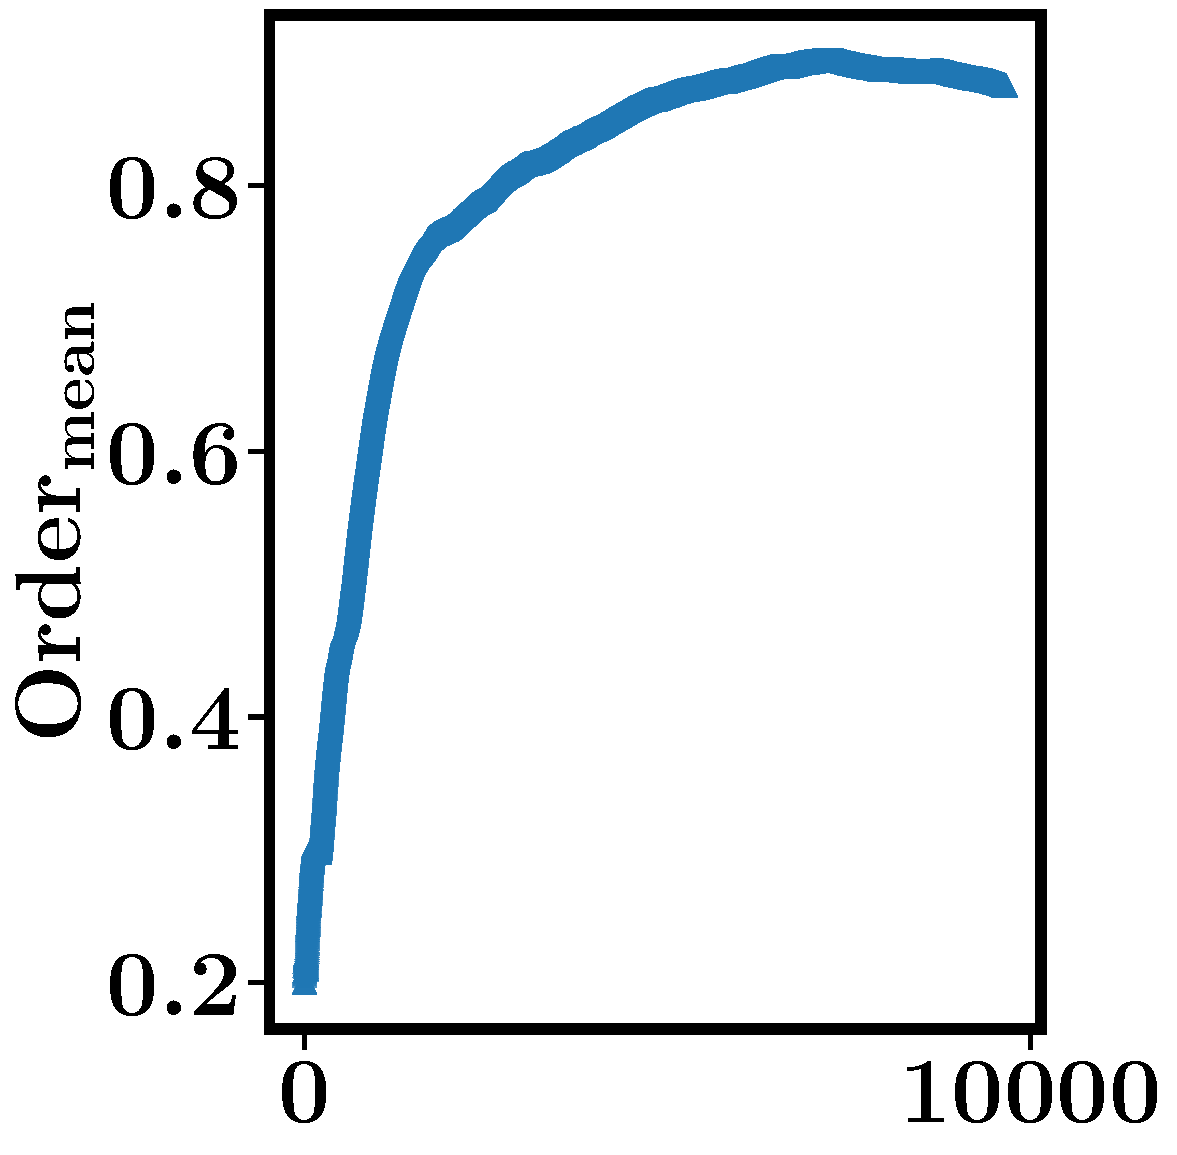
\includegraphics[width=\textwidth]{figures/plot_order_T0-5.pdf}
    \caption{Average order for $T = 0.5 < T_c$.}
     \label{fig:E0.5}
\end{figure}


\begin{figure}[ht]
  \centering
    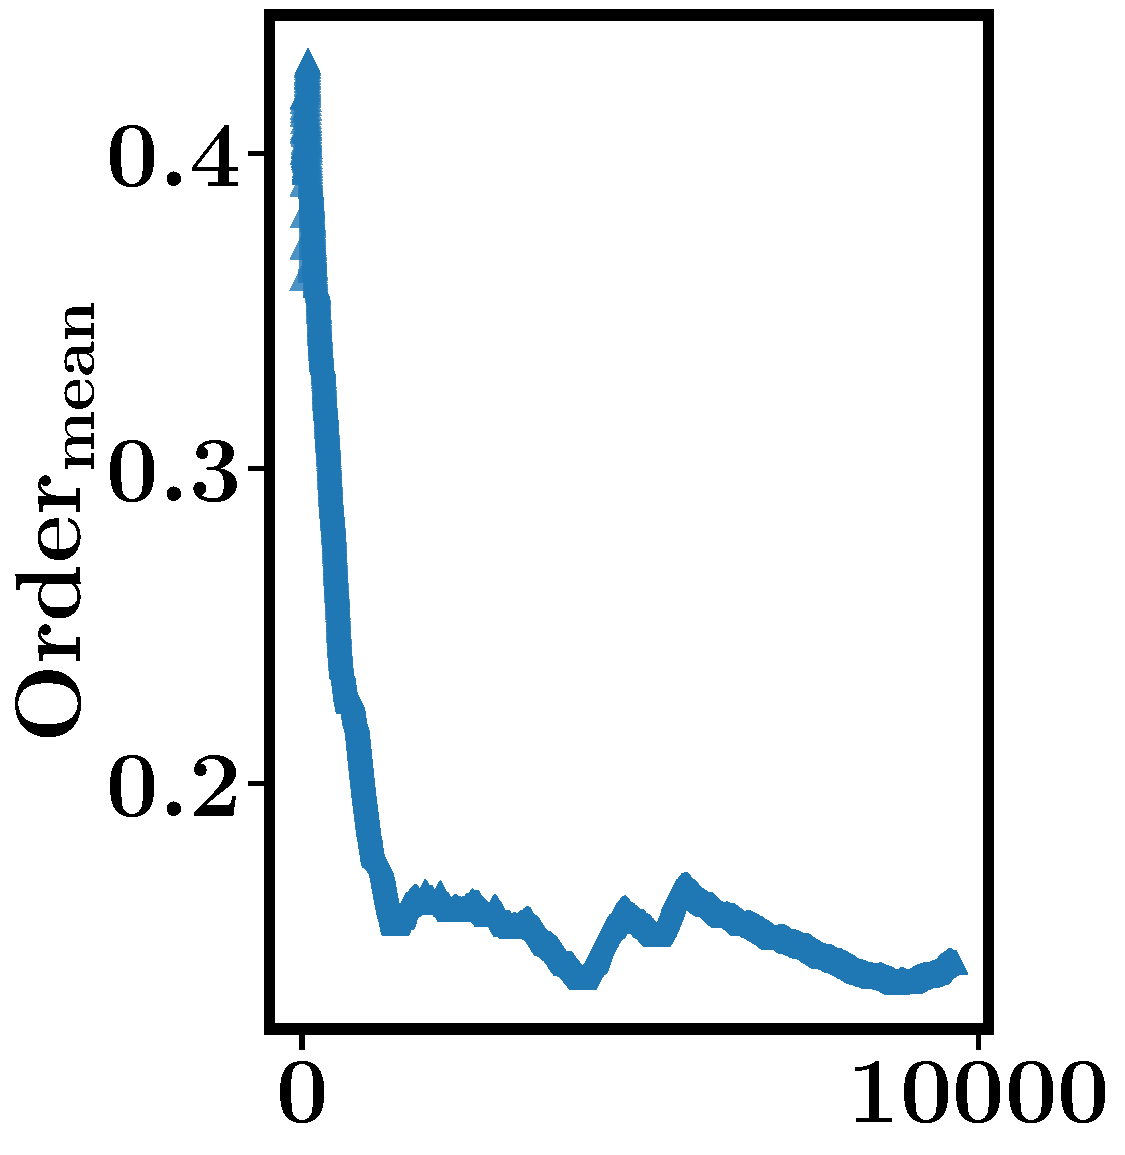
\includegraphics[width=\textwidth]{figures/plot_order_T1-134593.pdf}
    \caption{Average order for $T = 1.134593 = T_c$.}
     \label{fig:E0.5}
\end{figure}


\begin{figure}[ht]
  \centering
    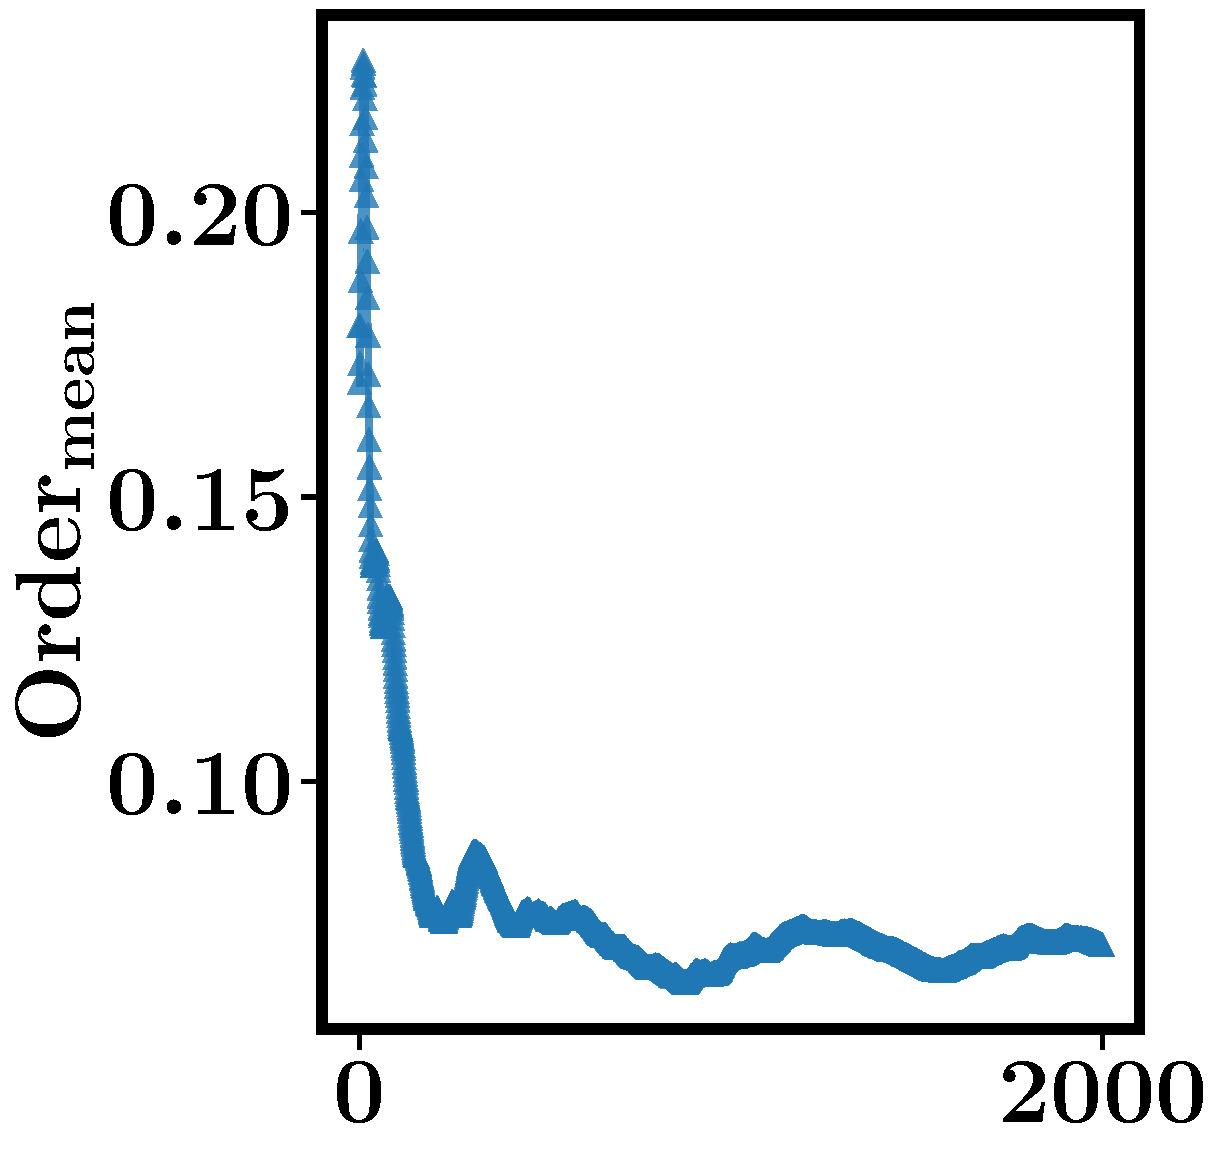
\includegraphics[width=\textwidth]{figures/plot_order_T5.pdf}
    \caption{Average order for $T = 5 > T_c$.}
     \label{fig:E0.5}
\end{figure}

% \begin{figure}[ht]
%   \centering
%     \includegraphics[width=\textwidth]{another_workflow.pdf}
%     \caption{Workflow for homogenized cross-section generation}
%      \label{fig:gen_workflow}
% \end{figure}

% \begin{figure}[ht]
%   \centering
%     \includegraphics[width=\textwidth]{another_workflow.pdf}
%     \caption{Workflow for homogenized cross-section generation}
%      \label{fig:gen_workflow}
% \end{figure}



\newpage
\newpage
\appendix
\begin{appendix}
\newpage
\code{cpp}{main.cpp}{Main Executable}{main}
\newpage
\code{cpp}{physics.hpp}{Monte Carlo Class header file}{mch}
\newpage
\code{cpp}{physics.cpp}{Monte Carlo Class definitions}{mc}
\newpage
\code{cpp}{io.cpp}{Read/Write Class definitions}{io}
\newpage
\code{make}{Makefile}{Makefile.}{make}
\newpage
\code{python}{plot.py}{Plotting Function}{plot}
\end{appendix}
%%%%%%%%%%%%%%%%%%%%%%%%%%%%%%%%%%%%%%%%%%%%%%%%
% \newpage
% \bibliographystyle{unsrt}
% \bibliography{mduschen_Ex1.bib}

\end{document}